\section{Design and Implmentation}\label{sec:design_and_implmentation}

\subsection{System Architecture}\label{subsec:system_architecture}

The goal of the system is to be used by non-technical users. The system consists of three processes or modules. These processes are the training process, selection process, and prediction process. The first two processes interact with each other. Their task is to produce the best-suited model for the user's needs. The third process interacts with the selected models to generate the predictions. \autoref{fig:system_architecture}, shows the architecture of the system. The user is indirectly allowed to access the training and prediction process. The user data is stored on a local drive for easier and faster access.

\begin{figure}[ht]
    \centering
    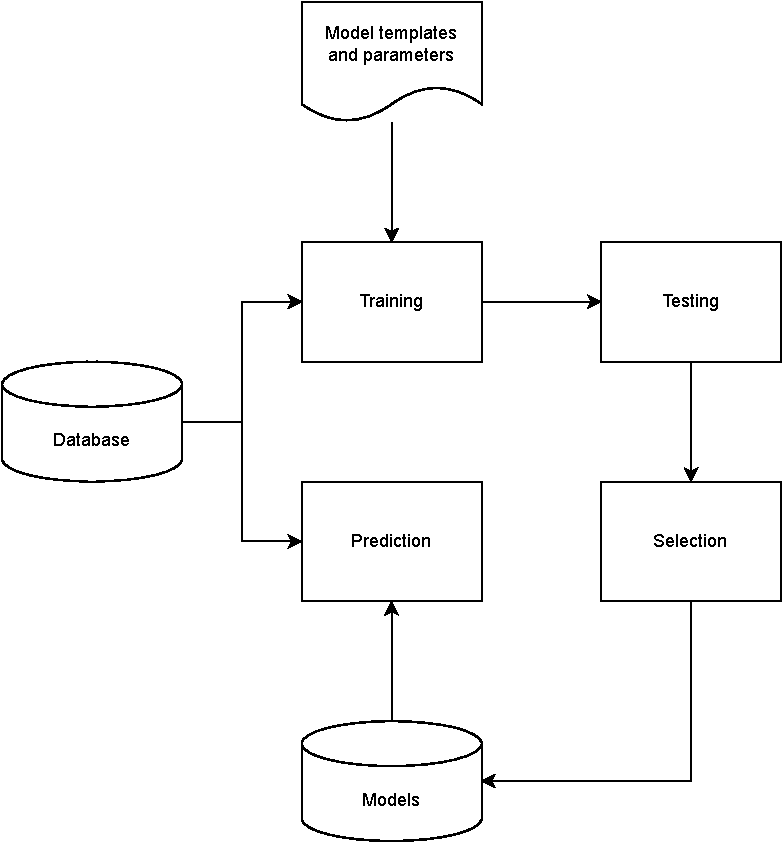
\includegraphics[width=0.9\columnwidth]{media/sec03/system_architecture.pdf}
    \caption{System Architecture}
    \label{fig:system_architecture}
\end{figure}

\subsection{System Processes}\label{subsec:system_processes}

As stated in previous section, the system consists of three primary processes. These processes are the training process, selection process, and prediction process. These processes are described in the following sections.

\subsubsection{Training Process}\label{subsubsec:training_process}

The training process is the first process in the system. \autoref{fig:training_process}, shows the structure of the training process. The training process has many functions. The first function is gathering data from the user and pre-processing it for training purposes. The training process also generates models with the template, which contains model structure and parameters. These models are trained with processed data and stored for future use. The performance of models is also calculated during this phase and store for selection purpose.

\begin{figure}[ht]
    \centering
    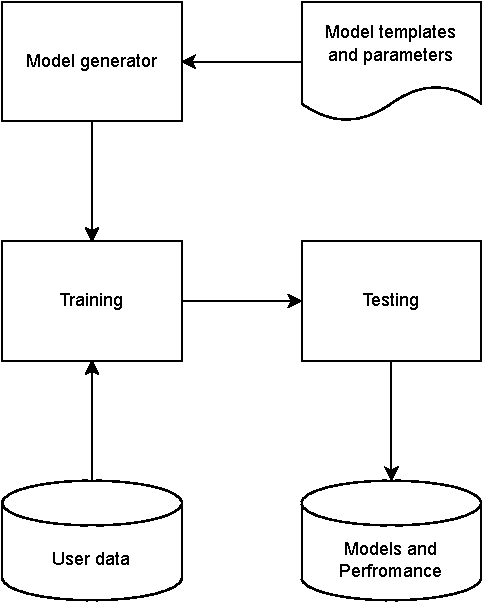
\includegraphics[width=0.6\columnwidth]{media/sec03/training_and_testing.pdf}
    \caption{Training Process}
    \label{fig:training_process}
\end{figure}

\subsubsection{Selection Process}\label{subsubsec:selection_process}

The selection process is second in the system. \autoref{fig:selection_process}, shows the structure of the training process. This process evaluates the performance of models based on metrics and weightage. The metrics of models are generated during the training process. The performance weightage is defined by the user depending on requirements. The final performance score is calculated and used for selection of the best model for users task. The selected model is stored in a separate directory with a label for easier access. This model will be used for prediction problems.

\begin{figure}[ht]
    \centering
    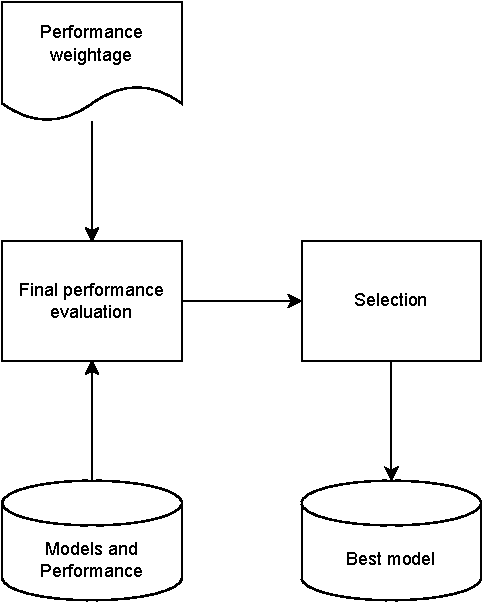
\includegraphics[width=0.6\columnwidth]{media/sec03/selection.pdf}
    \caption{Selection Process}
    \label{fig:selection_process}
\end{figure}

\subsubsection{Prediction Process}\label{subsubsec:prediction_process}

The prediction process is the final process in the system. \autoref{fig:prediction_process}, shows the structure of the prediction process. This process unpacks the best model and loads it for prediction. The model generates predictions with user-provided data. The output is displayed to the user. This output is also stored for future reference.

\begin{figure}[ht]
    \centering
    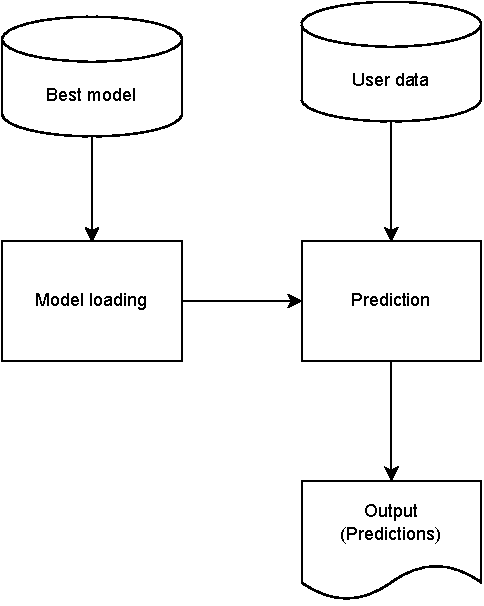
\includegraphics[width=0.6\columnwidth]{media/sec03/prediction.pdf}
    \caption{Prediction Process}
    \label{fig:prediction_process}
\end{figure}

\subsection{Algorithms}\label{subsec:algorithms}

The system uses two algorithms to run. These algorithms are training and selection algorithms and prediction algorithms.

\vspace{-0.5em}
\subsubsection*{Training and Selection Algorithm}\label{subsubsec:training_and_selection_algorithm}
\vspace{0.5em}
\begin{enumerate}
    \item Collect/Receive dataset.
    \item Split data into 80:20 ratio for training and testing.
    \item Build a model from presets.
    \item Train models with training dataset and store models.
    \item Evaluate the performance of models with the testing dataset.
    \item Rank models with help of performance and premade tuning parameters.
    \item Selects the best model and stores it for future use.
\end{enumerate}

\vspace{-0.5em}
\subsubsection*{Prediction Algorithm}\label{subsubsec:prediction_algorithm}
\vspace{0.5em}
\begin{enumerate}
    \item Collect/Receive dataset.
    \item Load best-suited model data from the storage.
    \item Unpack model for predictions.
    \item Make predictions with the provided dataset and loaded model.
    \item Return predictions to user.
\end{enumerate}

\subsection{Implmentation}\label{subsec:implmentation}

\subsubsection{Web Architecture}\label{subsubsec:web_architecture}

The system provides service with a web application. The users aren't allowed to interact with the system directly. This provision is to provide security and reduce the outside influence on results. The interface layer is used for a user to interact with the system indirectly. \autoref{fig:web_architecture}, shows the web architecture of the system. The system is connected to the database directly. A direct connection is provided to access live data. User-provided data is processed by the system and stored in the database.

\begin{figure}[ht]
    \centering
    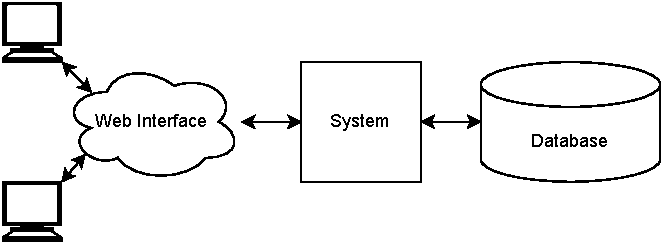
\includegraphics[width=0.9\columnwidth]{media/sec03/web_architecture.pdf}
    \caption{Web Architecture}
    \label{fig:web_architecture}
\end{figure}

\subsubsection*{Web Interface}\label{subsubsec:web_interface}
The web interface provides users with a way to interact with the system. The primary function of the web interface is to provide secure access to the system process. Approved users can interact with various modules on the system. This interface allows users to access selection and prediction processes. Users can upload data to the system.

The interface presents prediction results as well as performance evaluation results. Prediction results are provided in tabular format and stored in CSV files for future reference. Performance results are presented in graphical format and also stored in CSV files for future reference.
